\chapter{Kadane on Skill, Chance and the Expert Witness}
\label{ch:kadane}

\section{The working Bayesian}

Joseph Kadane, for many years at Carnegie Mellon, is a Bayesian statistician who has spent a substantial part of his career as an expert witness and consultant in litigation. His casebook \emph{Statistics in the Law} collects many of these engagements with the court documents and commentary: whether electronic draw poker requires skill, the composition of juries, an allegation of copying in an examination, sampling in tax audits, crossing lines in a patent case, the New Jersey Turnpike stops, and others \citep{kadane2008}. His textbook \emph{Principles of Uncertainty} sets out the subjective Bayesian foundations he applies \citep{kadane2011}. With David Schum he produced the probabilistic analysis of the Sacco and Vanzetti evidence discussed in Chapter~\ref{ch:graphs} \citep{kadane_schum1996}.\index{Kadane, Joseph}

Kadane's legal work is instructive because it shows a Bayesian statistician doing the ordinary work of an expert: defining the question in a way the law can use, collecting data, choosing a model the court can understand, and defending conclusions under cross examination. It shows that Bayesian analysis is not only a philosophy of evidence but a practical tool. This chapter concentrates on his work on games of skill and chance, which raises a legal question with a clean statistical structure, and then surveys his other engagements.

\section{Skill and chance in the law}

Gambling is regulated or prohibited in most jurisdictions, and the definition of gambling usually turns on chance. A wager on a game of chance is gambling; a contest of skill with a prize is not. Most games involve both. Courts have adopted several tests to classify them.\index{games of skill}

\begin{description}
\item[Dominant factor test] A game is gambling if chance predominates over skill in determining the outcome. Most American states use some form of this test.
\item[Material element test] A game is gambling if chance is a material element in determining the outcome, even if skill predominates. Some states use this stricter test.
\item[Any chance test] A game is gambling if chance plays any part. Few jurisdictions apply this literally, since almost every contest has some element of luck.
\end{description}
None of these tests says how to measure the contributions of skill and chance. That is a statistical question, and it was the question Kadane was asked in a case about electronic draw poker machines in the 1980s.

\section{Electronic draw poker}

An electronic draw poker machine deals a player five cards; the player chooses which to hold and which to discard; the machine replaces the discards; and the final hand determines the payout according to a fixed table. The cards are dealt at random. The player's only decisions are which cards to hold. Is this a game of skill?

Kadane's approach, described in his contribution to the volume \emph{Statistics and the Law} and reproduced in his casebook, was to compare the results of two strategies \citep{kadane1986,kadane2008}. A dumb strategy, representing a player with no skill, makes the choice of cards to hold at random or by a naive rule. A smart strategy chooses the hold that maximises expected payout. If skill matters, the smart strategy should do much better than the dumb one. Kadane computed, for the payout table at issue, the expected return of each strategy, and found that the smart strategy's expected return was far better than the dumb one's. Choices made a large difference to outcomes, so the game involved substantial skill.

John Lehoczky's comment, and Kadane's rejoinder, both reproduced in the casebook, debated whether this comparison answered the legal question. Even the smart strategy might lose money on average, since the machines are designed to favour the house. Does a game in which skill reduces losses but cannot produce gains count as a game of skill? Kadane's position was that the dominant factor test asks whether skill or chance determines the outcome, not whether a player can win, and that a large difference between strategies shows that outcomes depend substantially on skill. Ware and Kadane developed the analysis further \citep{kadane2008}.

\section{Measuring skill: a Bayesian framework}

The skill question can be put in terms of variance. Let $Y_{ij}$ be the result of player $i$ in hand $j$. A simple random effects model writes
\begin{equation}
Y_{ij} = \mu + \alpha_i + \epsilon_{ij}, \qquad \alpha_i \sim N(0, \sigma_\alpha^2), \quad \epsilon_{ij}\sim N(0,\sigma_\epsilon^2),
\label{eq:skillmodel}
\end{equation}
where $\alpha_i$ is player $i$'s skill and $\epsilon_{ij}$ is luck. In a single hand, the share of variance due to skill is $\sigma_\alpha^2/(\sigma_\alpha^2 + \sigma_\epsilon^2)$. Over $m$ hands, the variance of a player's average result due to luck falls to $\sigma_\epsilon^2/m$, so the share due to skill rises to
\begin{equation}
s(m) = \frac{\sigma_\alpha^2}{\sigma_\alpha^2 + \sigma_\epsilon^2/m}.
\label{eq:skillshare}
\end{equation}
Skill accounts for half the variance when $m = \sigma_\epsilon^2/\sigma_\alpha^2$.
Figure~\ref{fig:skill} plots $s(m)$ for several values of skill variance. Under this model every game with $\sigma_\alpha^2 > 0$ becomes predominantly a game of skill if played long enough. Whether a game is predominantly skill or chance therefore depends on the horizon over which the outcome is judged: a single hand, a session, or a career.\index{skill share}

\begin{figure}[t]
\centering
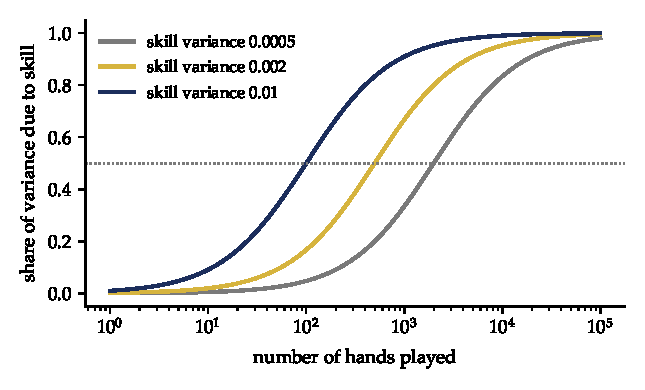
\includegraphics[width=\linewidth]{fig_skill}
\caption{Share of the variance of a player's average result attributable to skill, as a function of the number of hands played, for three levels of skill variance relative to unit luck variance per hand.}
\label{fig:skill}
\end{figure}

This is the crux of many legal disputes over poker. In a single hand of Texas Hold'em, luck plays a large role; a weak player with a strong hand beats a strong player with a weak one. Over thousands of hands, the stronger player wins reliably. Courts that have asked whether chance swamps skill in a single hand have often found poker a game of chance, as the North Carolina Court of Appeals did in \emph{Joker Club v Hardin} in 2007; analyses that look at repeated play find it a game of skill, and Judge Weinstein reached that view in \emph{DiCristina}, discussed below. Courts have split. Miles, Levitt and Rosenfield argued in the \emph{Georgetown Law Journal} that the single hand conception is unduly narrow \citep{miles2013}. Levitt and Miles, using data from the World Series of Poker, showed that players identified in advance as highly skilled earned substantially higher returns than others \citep{levitt2014}.

The Bayesian contribution is to estimate $\sigma_\alpha^2$ and the individual $\alpha_i$ with appropriate uncertainty, using a hierarchical model, and to report the posterior distribution of $s(m)$ for the horizon the law considers relevant. A court can then choose the horizon, which is a legal question, and the statistician can report the skill share for that horizon, which is a factual one.

\section{Simplified poker and the theory of skill}

Larkey, Kadane, Austin and Zamir studied skill in a simplified poker game using computer tournaments among strategies of different sophistication \citep{larkey1997}. A strategy that played randomly, representing zero skill, performed worst; more sophisticated strategies, which took account of the opponent's likely holdings and betting, performed progressively better. Their paper made a conceptual point that is easy to miss: skill in games is relative. A strategy's success depends on the strategies of the other players. A game can reward skill even when no strategy guarantees a profit against every opponent, because a skilled player profits against unskilled ones. In poker, the house takes a fee and players play against each other, so the distribution of skill among players determines who wins.

\section{United States v DiCristina}

\begin{casebox}{United States v DiCristina}
Lawrence DiCristina operated a poker room in Staten Island and was charged under the federal Illegal Gambling Business Act, which applies to businesses that conduct illegal gambling under state law. In 2012 Judge Jack Weinstein of the Eastern District of New York, after hearing extensive expert testimony on skill in poker, including statistical analysis of a large number of online hands, held that poker was predominantly a game of skill and was not gambling within the meaning of the federal statute, and set aside the conviction \citep{dicristina2012}. In 2013 the Second Circuit reversed, holding that the statute covered any business that violated state gambling law, and that poker games of the kind at issue violated New York law, without needing to decide whether poker was a game of skill \citep{dicristina2013}.
\end{casebox}

\emph{DiCristina} shows both the power and the limits of statistical evidence on skill. Judge Weinstein, whose survey of his colleagues on reasonable doubt we met in Chapter~\ref{ch:standards}, engaged with the evidence in detail and was persuaded. The appellate court decided the case on statutory grounds that made the evidence irrelevant. The statistician can answer the factual question, but the legal question of which factual question matters belongs to the courts.

\section{Fantasy sports and online games}

The same issues arose with daily fantasy sports in the 2010s. Operators argued that selecting a fantasy team requires skill and pointed to evidence that a small fraction of players won most of the prizes. Regulators and some courts argued that the outcome of any single contest depends heavily on the unpredictable performance of athletes. In New York, the legislature authorised and regulated interactive fantasy sports in 2016; in 2022 the state's highest court, by a 4 to 3 vote, upheld that legislation against a constitutional challenge, accepting the legislature's judgment that such contests are not gambling within the meaning of the state constitution \citep{white2022}. Three judges dissented. The statistical evidence on skill was relevant but not decisive.

India illustrates a different path. Indian law has long distinguished games of skill from gambling. The Supreme Court held in 1968 that rummy is a game mainly and preponderantly of skill \citep{satyanarayana1968}, and in 1996 that horse racing is a game of skill, so that wagering on it is not gambling \citep{lakshmanan1996}. These decisions were relied on by the online gaming industry, which grew rapidly. In 2025 Parliament enacted legislation prohibiting online money games regardless of whether they involve skill or chance, while promoting other forms of online gaming. The legislature replaced a factual test that courts had applied case by case with a categorical rule. In decision theoretic terms, the legislature can be read as judging that the cost of classification errors and the social harms of money games outweighed the benefit of permitting skill games for money.\index{India!online gaming}

\section{Kadane's other engagements}

\subsection{Jury challenges and peremptory strikes}

Kadane's casebook includes an analysis of a jury challenge in Indiana, \emph{Azania v State}, decided by the Indiana Supreme Court in 2002 on a successive post-conviction petition in a death sentence case, in which the defendant argued that the county jury pool systematically excluded black jurors. The analysis compared the observed representation of black jurors with the expected representation under the selection procedure, taking account of the stages of selection at which under representation could arise \citep{kadane2008}. With Roth and DeGroot, Kadane earlier analysed the sequential game of peremptory challenges, in which prosecution and defence alternately strike prospective jurors without cause, and derived optimal strategies under assumptions about each side's beliefs about jurors' leanings \citep{roth1977}. The analysis showed that the order and number of strikes interact with the parties' information in ways that can be modelled as a Bayesian sequential decision problem. The Supreme Court's later decision in \emph{Batson v Kentucky}, forbidding race based peremptory strikes, created a further statistical question: how to infer discriminatory intent from a pattern of strikes.\index{peremptory challenges}

\subsection{Driving while black}

In \emph{State v Soto}, a New Jersey trial court in 1996 granted motions to suppress evidence obtained in stops of black motorists on the New Jersey Turnpike, finding a pattern of racial targeting \citep{soto1996}. The evidence included surveys of the racial composition of motorists on the turnpike and of those who were speeding, compared with the composition of those stopped. A difficulty was missing data: the race of many stopped motorists was not recorded. Kadane and Terrin analysed the problem of missing data in this context, showing how assumptions about the missing records affected the conclusion and how a Bayesian analysis could represent uncertainty about them \citep{kadane1997}. Their analysis found that the conclusion of disproportionate stops was robust across a wide range of assumptions about the missing data, which is exactly the kind of sensitivity analysis Fienberg and Kadane had recommended in 1983 \citep{fienberg_kadane1983} (Chapter~\ref{ch:fienberg}).\index{State v Soto}

\subsection{Hierarchical models for employment}

Kadane and Woodworth developed hierarchical Bayesian models for employment discrimination cases, in which decisions such as promotions or terminations are made by many decision makers in many units of a firm \citep{kadane2004}. A hierarchical model lets the analyst estimate the effect of a protected characteristic while allowing for variation across units, and can distinguish a firm wide policy from the actions of particular managers. This matters legally, because disparate treatment by a few managers may support individual claims but not a pattern or practice claim. The Supreme Court's decision in \emph{Wal Mart Stores v Dukes}, which rejected class certification in a nationwide sex discrimination case because the plaintiffs had not shown significant proof of a general policy of discrimination, as Rule 23(a)(2) commonality required, turned on exactly this question of whether the variation was firm wide or local.

\subsection{Tax audits and sampling}

With Bright and Nagin, Kadane analysed the use of statistical sampling in tax audits, where an auditor examines a sample of a taxpayer's transactions and extrapolates the error rate to the whole \citep{bright1988}. The legal question is how much the taxpayer should owe given sampling uncertainty. A point estimate overcharges about half the time; a lower confidence bound protects the taxpayer at the cost of undercollection. The decision theoretic answer depends on the relative losses of over and under collection, which is a policy question, but the analysis makes the trade off explicit.

\section{Lessons for the expert witness}

Kadane's career suggests several lessons for statisticians who give evidence.

First, define the question in the law's terms. The court does not need a posterior probability of guilt. It needs an answer to a specific question that the law makes relevant, such as whether skill predominates or whether a disparity is likely due to chance. The statistician's first job is to translate.

Second, use simple models the court can follow, and show that the conclusion is robust to reasonable departures from them. Kadane's poker analysis compared two strategies; his turnpike analysis varied the treatment of missing data. For the turnpike the robustness check carried as much weight as the main result.

Third, be open about the prior. Kadane and Schum reported their separate assessments in the Sacco and Vanzetti analysis. An expert who reports only one prior invites the cross examiner to ask why that one.

Fourth, accept that the law may decide the case on other grounds. \emph{DiCristina} was reversed on the statute; the census case in Chapter~\ref{ch:fienberg} was decided on statutory interpretation. Statistical evidence informs legal decisions but does not dictate them.

\section*{Notes and Questions}
\addcontentsline{toc}{section}{Notes and Questions}
\begin{enumerate}[label=\arabic*.]
\item Using \eqref{eq:skillshare} with $\sigma_\epsilon^2 = 1$ per hand, find the number of hands at which skill accounts for half the variance when $\sigma_\alpha^2 = 0.002$. Should a court assess skill over one hand, one session of three hundred hands, or a year?
\item Design a study to measure skill in a fantasy sports contest. What data would you need, and what model would you fit?
\item In electronic draw poker the house may have an edge even against the optimal strategy. Does this matter under the dominant factor test? Under the material element test?
\item The Indian Supreme Court found rummy to be a game of skill. If you were asked to give evidence, how would you measure skill in rummy?
\item In a pattern of peremptory strikes, a prosecutor strikes four of five black venire members and two of twenty white ones. Formulate a Bayesian test of the hypothesis that race influenced the strikes. What alternative explanations should the model include?
\item Read the casebook materials on electronic draw poker, including Lehoczky's comment and Kadane's rejoinder. Whose argument do you find more persuasive, and why?
\end{enumerate}

\section*{Further reading}
Kadane's \emph{Statistics in the Law} \citep{kadane2008} and \emph{Principles of Uncertainty} \citep{kadane2011}; Larkey, Kadane, Austin and Zamir on skill in games \citep{larkey1997}; Levitt and Miles on poker \citep{levitt2014}.
